\section*{Úvod}

Řadu fyzikálních, chemických, biologických nebo socio-ekonomických procesů lze popsat pomocí obyčejných nebo parciálních diferenciálních rovnic (ODR, PDR) a jejich soustav.
Řešení těchto rovnic umožňuje predikci a optimalizaci příslušných procesů při řešení řady inženýrských problémů jako např. vedení tepla, proudění kapalin a plynů, statické a dynamické namáhání konstrukcí nebo vývoj populace živých organismů.
PDR jsou rovnice, kde neznámou je fyzikální pole popsané funkcí $u(\vc x)$, která bodům $\vc x$ na na nějaké prostorové oblasti přiřazuje hodnoty pole. 
Pro většinu PDR nelze řešení (funkci) zapsat v uzavřeném tvaru (t.j. pomocí analytických vzorců), proto jsou využívány numerické (přibližné) metody, jejichž výsledkem je funkce splňující rovnici 
s nějakou numerickou chybou.
Je to obdobné jako nemožnost reprezentovat v počítači přesně reálná čísla.

Metoda konečných prvků -- MKP, anglicky Finite Elment Method (FEM) je jednou ze standarodních metod pro numerické (přibližné) řešení PDR, dalšími metodami jsou například metoda konečných objemů (Finite Volume Method -- FVM) nebo nespojitá Galerkinova metoda (Discontinuous Galerkin -- DG).
Společným rysem těchto metod je využití takzvané slabé formulace zadané rovnice. 

V tomto textu představíme některé typy diferenciálních rovnic, které se používají pro popis výše zmíněných procesů, a jejich klasickou a slabou formulaci.
Na modelové úloze (eliptická rovnice pro popis jednorozměrného vedení tepla) si ukážeme postup metody konečných prvků v případě tzv. lineárních prvků.
Pro zobecnění metody zavedeme potřebný matematický aparát.
Ten nám umožní aplikovat MKP pro širokou řadu problémů a analyzovat důležité vlastnosti metody, zejména pak konvergenci a chybu přibližného řešení.
Důraz je kladen také na praktickou implementaci metody v MATLABu nebo jiném vhodném programovacím jazyce.




\section{Klasifikace PDR}
\subsection{Fyzikální pole}
\begin{itemize}
 \item většinou abstrakce průměrování veličin mikrosvěta:
 \begin{itemize}
    \item koncentrace ($(0,1)$)
    \item teplota - průměrná kinetická energie částic, $ E = \frac{3}{2}T k_B$
    \item tlak / tlaková výška kapaliny v porézním médiu - průměrování sil při kolizích mezi částicemi
    \item elastické napětí - průměrná síla mezi částicemi
 \end{itemize}
 \item vektorová pole - většinou odvozená od závislosti skalárních veličin na prostoru
 \begin{itemize}
    \item poloha, rychlost, zrychlení
    \item gradient
    \item síla - vztažená ke zrychlení
    \item elektrická a magnetická intenzita - hustota elektrických a magnetických sil (opět vztaženo ke zrychlení)
    \item hustota toku $\vc q_u$ skalární veličiny $u$ - jaké množství veličiny $u$ přeteče za 
    jednotku času (sekundu)
          přes jednotkové plochy s normálami $X$, $Y$, $Z$.\\
          Pro obecnou jednotkovou plochu s normálou $\vc n$ je $q_u \cdot n$ skalární veličina 
          udávající kolik přeteče pře tuto plochu za jednotku času.          
 \end{itemize}

 \item tenzorová pole - abstraktní, vyjádření lineární závislosti vektorových veličin\\
 
 \begin{itemize}
    \item gradient vektorové veličiny - nesymetrický tenzor
    \item tenzor napětí - závislost síly na orientaci plochy na kterou síla působí, zahrnuje kolmou sílu (tlak/tah) i smykové síly.
    \item Závislost toku veličiny $q_u$ na gradientu veličiny $u$. Pro veličiny založené na průměrování mikrosvěta odpovídá tento tok difúzi. 
          Interagující částice vedou k vyrovnání hodnot veličiny $u$ (např. teploty) v prostoru.
          Tento tok je tedy proti směru gradientu:
          $$
          \vc q_u = -k \grad u
          $$
          Veličinu $k$ ozančujeme jako {\it vodivost}, např. tepelná vodivost, 
          hydraulická vodivost, elektrická vodivost. Pro transport látek mluvíme však o {\it difusivitě}
          nebo keoficientu hydrodynamické disperze. Pokud je materiál anisotropní,
          nelze tento vztah zapsat pomocí skalární vodivosti $k$, resp. existují tři kolmé 
          směry (vlastní vektory) ve kterých vztah platí pro tři vodivosti (vlastní čísla).
          Obecně je vztah popsán tenzorem (maticí $3\times 3$) $\tn K$:
          $$
          \vc q_u = - \tn K \grad u.
          $$
          
          
          Tento tenzor vodivosti (nebo např. tenzor hydrodynamické disperze) popisuje
          {\it anisotropii materiálu} tedy závislost chování na směru.
  \end{itemize}
\end{itemize}

Matematicky, pole jako funkce prostoru (a času).

\subsection{Advekčně - difúzní rovnice}
 \begin{itemize}
    \item zákony zachování pro veličinu $u$ s tokem $\vc q(u)$ $\Longrightarrow$:
        $$\prtl_t u(t, \vc x) + \div \vc q(u)(t, \vc x) = 0$$
    \item Celkový tok veličiny zahrnuje advekční a difźní část:
    $$
    \vc q_u = \vc q_a + \vc q_d
    $$
    \item advekční tok $\vc q_a$ (unášení médiem, rychlostní pole $V$):
        $$\vc q_a(t, \vc x) = u(t, \vc x) \vc V(t, \vc x) $$
    \item difúzní tok (viz. výše, statistika interakcí částic)
  \end{itemize}

\subsubsection{Rovnice vedení tepla}
Pojďme se podívat jak asi bude vypadat příslušná rovnice - vedení tepla. 
První otázka je, jak matematicky popsat rozložení teploty na tělese. Lze např. 
na profil umístit čidla teploty a popsat rozložení teploty pomocí vektoru teplot 
na čidlech. Pro malý počet čidel nám bude chybět informace o teplotě mezi čidly. 
Pokud budeme zvyšovat počet čidel můžeme si představit, že známe teplotu v každém 
bodě, takže teplota bude funkce, která bodu $\vc x$ v oblasti tělesa $\Omega$ přiřazuje 
$u(\vc x)$. Ovšem toto je pouze aproximace reality, např. pojem teplota dává smysl jen 
pro dostatečně velké soubory atomů.

Jaké rovnice určují tepotní pole $u(x)$? Jednak zde máme princip zachování energie,
zde to znamená, že celkový teplný tok přes hranici každé oblasti $M \subset \Omega$
bude nulový a použitím Gaussovy věty máme:

\[
    \int_{\prtl M} \vc j \cdot \vc n \d S = \int_{M} \div \vc j \d x = 0
\]

Obecně by na oblasti mohl být nějaký tepelný zdroj daný objemovou hustotou
tepelného toku $f(x)$ $[W/m^3]$, resp. $[W/m^2]$ pro 2d. Pak celkový tok přes hranici 
bude roven celkovému objemovému teplu:

\[
    \int_{\prtl M} \vc j \cdot \vc n \d S = \int_{M} \div \vc j \d x = \int_{M} f \d x
\]

Pokud tato rovnice platí pro všechny otevřené množiny $M$, platí také pro libovolně malé koule 
okolo každého bodu, pokud jsou funkce pod objemovým integrálem spojité, tak platí bodová 
forma rovnice:
\[
    \div \vc j = f
\]


Teplený tok $\vc j(\vc x)$ je vektorové pole, které je dané Fourierovým zákonem:
\[
   \vc j = - k \grad u 
\]

To je zápis poznatku, že teplo se předává z místa s vyšší teplotou na místo s nižší 
teplotou a to úměrně rozdílu teplot a tepelné vodivosti $k$. Pokud si představíme 
materiál, který je složen ze střídajících se vodivých a nevodivých vrstev, 
např. hliníková fólie a texílie. Bude teplná vodivost vyšší ve tečném směru a 
vyšší v komém směru. Celkově se teplo nebude šířit vždy ve směru 
gradientu a tepelnou vodivost můžeme reprezentovat tenzorem:

\[
   \vc j = -\tn K \grad u,\quad \tn K = \tn Q^T \tn{ \Lambda} \tn Q
\]

Obecně si akci tenzoru můžeme rozložit na rotaci vektoru (gradientu) do jiné kartézské soustavy, 
následně přenásobení jednotlivých složek teplnými vodivostmi (3 vlastní čísla tenzoru)
a rotace zpět do původní soustavy. Matice rotace $Q$ rotuje ortonormální bázi 
$\vc e_1, \vc e_2, \vc e_3$ na jinou ortonormální bázi tvořenou sloupcovými vektory matice.
To že je nová báze ortonormální znamená že pro dva různé sloupcové vektory je skalární 
součin $0$ a pro stejné e součin $1$, tedy  $Q^TQ = \tn E$, což znamená, že 
inverze rotaze je její transpozice. Jelikož vlastní čísla, t.j. vodivosti 
jsou kladné, je $\tn K$ pozitivně definitní matice.

Celkem tedy dostáváme rovnici:
\[
    - \div\left( \tn K \grad u \right) = f  
\]
v každém bodě oblasti $\Omega$. Touto rovnicí je dáno chování teploty uvnitř, 
ale nepopisuje interakci s okolím na hranici. Z matematického hlediska není řešení 
rovnice jednoznačné pokud nejsou na hranici předepsány tzv. okrajové podmínky.



\subsubsection{Eliptické rovnice}
Stacionární rovnice vedení tepla odvozená v předchozí kapitole je jedním z příkladů 
eliptických rovnic. To jsou rovnice s druhými derivacemi neznámé vůči prostorovým proměnným.
Je zde tedy podobnost s rovnicí elipsy:
\[
    ax^2 + by^2 = 1
\]


Základním příkladem je Laplaceova rovnice:
\[
    \Lapl u(\vc x) = 0
\]
respektive Poisonova rovnice
\[
    \Lapl u(\vc x) = f(\vc x).
\]

Obecná rovnice vedení tepla, pak popisuje též proudění vody v porézním prostředí 
(malá rychlost, zanedbatelná setrvačnost vody):
\[
   - \div( \tn K \grad p(\vc x)) = f(\vc x).
\]
v tomto kontextu je $\tn K$ tenzor hydraulické vodivosti a $p$ je piezometrická výška, t.j. 
diference vůču hydrostatickému tlaku. Další procesy popsané stejnou rovnicí: elektrický potenciál, 
difúze / disperze látek, jednoduchý model průhybu nosníku/desky.


Obecná rovnice druhého řádu:
\[
  \div\Big( \tn A \grad u(\vc x)\Big) + \vc b \grad u(\vc x) + c u(\vc x)= f(\vc x)
\]
je eliptická, pokud $\tn A$ je symetrická pozitivně definitní matice 
a je výrazně větší než-li $\vc b$ a $c$ (vyjasníme později).

Pro eliptické rovnice platí tzv. princip maxima. 
Pokud $u$ je řešením eplitické rovnice na oblasti $\Omega$
pak 
\[
    \max_{\vc x \in \Omega} u(\vc x) \le \max_{\vc x \in \prtl \Omega}  u(\vc x).
\]
Podobně pro minimum:
\[
    \min_{\vc x \in \Omega} u(\vc x) \ge \min_{\vc x \in \prtl \Omega}  u(\vc x).
\]
Ovšem pokud je $u$ řešením na $\Omega$, pak je řešením také na všech 
podoblastech a i na nich platí princip maxima/minima. Pojmem {\it oblast}
se myslí otevřená množina, topologicky ekvivalentní s kruhem/koulí, t.j. ``množina bez děr''.
Otevřená množina neobsahuje svoji hranici, kterou značíme $\prtl \Omega$. 
Naopak uzavřená množina obsahuje i svojí hranici. 


\subsubsection{Parabolické rovnice}
Příkladem parabolické rovnice je nestacionární rovnice vedení tepla:
\[
    \prtl_t(c \rho T) -\div(\tn K \grad T) = f
\]
Stejné příklady dalších procesů jako pro stacionární případ.

I zde platí princip maxima, ovšem se zahrnutím počáteční podmínky.
Označíme $\Omega_T = \Omega \times (0, T]$, tuto časoprostorovou oblast 
si můžeme představit jako válec, s podstavou $\Omega$ a s časem na vertikální ose. 
Počáteční čas $0$ a hranice $\prtl \Omega$ nejsou její součástí, ale koncový čas $T$
ano. Pro řešení parabolické rovnice na $\Omega_T$ platí:

\[
    \max_{(t, \vc x) \in \Omega_T} u(t, \vc x) \le \max_{(t, \vc x) \in \Gamma_T}  u(t, \vc x).
\]
... a podobně pro minimum. Zde $\Gamma_T$ je hranice $\Omega_T$ mimo koncového času, tedy 
$t=0$ nebo $\vc x \in \prtl \Omega$.

Parabolické rovnice zhlazují řešení v čase. Navíc pro libovolnou počáteční podmínku, nehladkou, s nespojitostmi. Je řešení po libovolně krátkém
čase již hladké v prostoru, byť třeba s velkými derivacemi. 

Vliv počátečních a okrajových podmínek se šíří nekonečnou rychlostí a okamžitě ovlivní celé řešení
nicméně vliv změny slábne exponenciálně se vzdáleností v čase a prostoru.
  
\subsection{Vlnové rovnice}
Příklady procesů s vlnovým charakterem řešení:
  \begin{itemize}
    \item vlny na hladině, viz. 
    \href{https://www.youtube.com/watch?v=6EKZKaWhufI}{``constructive interference'' example}
    \item zvuk, šíření v různých materiálech je dáno jejich mechanickými vlastnostimi\\
          aplikace:\\
          \href{https://en.wikipedia.org/wiki/Seismic_tomography}{seismiská tomografie}\\
          \href{https://en.wikipedia.org/wiki/Ultrasonic_testing}{ultrazvuková vyšetření a testování}\\
          \href{https://en.wikipedia.org/wiki/Acoustic_levitation}{Akustická levitace}
          a \href{https://www.youtube.com/watch?v=c05VSs3q56U&t=140s}{manipulace}\\
    \item Electromagnetické vlny: optika, rádiové vlny, ...\\
    Přenos signálu na extrémní vzdálenosti.\\
\href{https://en.wikipedia.org/wiki/Optical_tweezers}{Laserová pinzeta}\
     ...
     \end{itemize}

\subsubsection{Hyperbolické rovnice}
Typickým příkladem je jednoduchá vlnová rovnice struny:

\[
    \prtl_{tt} p(t, \vc x) = c^2 \Lapl p(t, \vc x)
\]

Transportní rovnice (rovnice kontinuity), např. pro rozpuštěnou látku:
\[
    \prtl_t (\rho c) + \div( (\rho c) \vc u)=0
\]

Eulerovy rovnice:
\[
    \prtl_t \rho + \div( \rho \vc u)=0
\]
\[
    \prtl_t (\rho \vc u_i) +\div(\rho \vc u_i \vc u) = - \grad P,
\]
Kvalitativní vlastnosti řešení:
\begin{itemize}
 \item Konečná rychlost šíření (vln).
 \item Nezhlazuje.  
 \item Nesplňuje princip maxima, řešení se může akumulovat v bodě 
 (součet vln).
\end{itemize}


\subsection{Vlnová rovnice (akustika)}
% Uvažujme materiál (tekutinu, nebo elastickou pevnou látku) s rychlostním polem  $u$. Ze zákona zachování hybnosti $\rho u$ 
% plyne použitím rovnice kontinuity:
% \[
%     \prtl_t (\rho \vc u_i) +\div(\rho \vc u_i \vc u) = - \grad P,
% \]
% kde $P$ je tlak, a jeho záporný gradient je hustota síly, která způsobuje změnu hybnosti podle 2. Newtonova zákona.
% Tato rovnice spolu s rovnicí kontinuity pro plyn:
% \[
%     \prtl_t \rho + \div( \rho \vc u)=0
% \]
% tvoří systém tzv. Eulerových rovnic popisujících proudění neviskózní stlačitelné tekutiny.

Odvodíme rovnici pro kmitání struny. Stav struny v čase $t$ a poloze $x$ je dán výchylkou struny $u(t,x)$. Pro zjendodušení si představujeme, 
že struna může kmitat jen v jednom směru. Na element daný intervalem $(a,b)$ působí síly v koncových bodech:
\[
    \vc F(t,a) = -T(t,a) \vc t(t,a),\quad \vc F(t,b) = T(t,b) \vc t(t, b)
\]
kde $T$ je napětí ve struně a $\vc t$ je tečný vektor $ t(t, x) = ( 1, \prtl_x u(t,x) )$. 
Jelikož v horizontálním směru se struna nepohybuje můsí být horizontální složka součtu sil rovna nule:
\[
    T(t,b) - T(t,a) = 0
\]
a jelikož jsme body $a$ a $b$ volili libovolně,  je napětí ve struně nazávislé na poloze: $T(t, x) = T(t)$.
Proto pro vertikální složku síly platí 
\[
    F_y = F_y(t,a) + F_y(t,b) = T(t)\big(\prtl_x u(t,b) - \prtl_x u(t,a)\big)
\]
Nyní použijeme 2. Newtonův zákon:
\[
    \frac{\d}{\dt} \int_a^b \rho(x) \prtl_t u(t,x) \d x = F_y(t,x) = T(t)\big(\prtl_x u(t,b) - \prtl_x u(t,a)\big) = T(t) \int_a^b \prtl_{xx} u(t,x) \d x 
\]
A jelikož $a$ a $b$ jsou libovolné, dostáváme bodovou rovnici:
\[
    \rho(x) \prtl_{tt} u(t,x) = T(t) \prtl_{xx} u(t,x) 
\]
Pokud předpokládáme konstantní hustotu $\rho(x) = \rho_0$ a zanedbáme změnu napětí struny při malé výchylce $T(t)=T_0$ dostaneme vlnovou rovnici ve tvaru:
\[
    \prtl_{tt} u(t,x) = c^2 \prtl_{xx} u(t,x)
\]
kde 
\[
    c=\sqrt{\frac{T_0}{\rho_0}}
\]
je rychlost šíření vlny. 
Mírně kompplikovanější je odvození vlnové rovnice pro změny (akustického) tlaku v prostoru:

\[
    \prtl_{tt} p(t, \vc x) = c^2 \Lapl p(t, \vc x)
\]
kde pro rychlost zvuku $c$ platí:
\[
    c = \sqrt{\frac{B}{\rho_0}},\quad B = \rho_0 \frac{\prtl P}{\prtl \rho}
\]
přičemž $B$ je objemová stlačitelnost při adiabatické expanzi. Pro vzduch máme $B=1.45\times 10^5\ Pa$ a hustotu $\rho_0 = 1.2kg/m^3$ a dostáváme rychlost zvuku:
\[
    c=347 \sqrt{\frac{kg.m/s^2/m^2}{kg/m^3}} = 1251 km/h
\]
Tabulková hodnota je $340m/s$.


\subsection{Experimenty}
Experimentujte s chováním parabolických a hyperbolických rovnic pomocí 
online \href{http://math.uchicago.edu/~luis/pde/heat.html}{řešiče rovnice vedení tepla}.
\begin{itemize}
 \item Ověřte si princip maxima vůči počáteční podmínce.
 \item Ověřte si princip maxima vůču okrajové podmínce.
 \item Ověřte zhlazování.
\end{itemize}

Experimentujte s chováním parabolických a hyperbolických rovnic pomocí 
online \href{http://math.uchicago.edu/~luis/pde/wave.html}{řešiče vlnové rovnice}.
\begin{itemize}
 \item Ověřte, že princip maxima neplatí. Nechte srazit dvě protichůdné vlny.
 \item Ověřte, že nedochází ke zhlazování.
\end{itemize}







  
%   
% \subsection{Úvodní příklad}
% Uvažujeme topidlo ve formě kanálu, které má efektivně předávat teplo 
% topného média okolnímu vzduchu o nižší teplotě.
% Topné médium proudí vnitřním kruhovým kanálem a tvar venkovní obálky
% je dán intervalem $y \in (-f(x), f(x))$. Pokud zanednáme konce kanálu, jsou parametry 
% problému stejné v každém kolmém řezu kanálu (viz. Obr. \ref{topeni2D} a Obr. 
% \ref{topeni2D}) a je tedy 
% možné řešit pouze 2D úlohu vedení tepla.
% 
% \begin{figure}
%  \center
%  \label{topeni2D_kulaty}
%  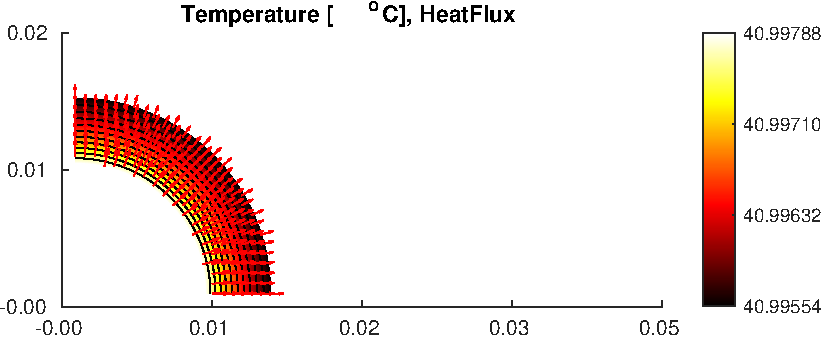
\includegraphics[width=0.8\textwidth]{flux_11.pdf}
%  \caption{Rozložení reploty pro kruhový průřez.}
% \end{figure}
% 
% \begin{figure}
%  \center 
%  \label{topeni2D_placaty}
%  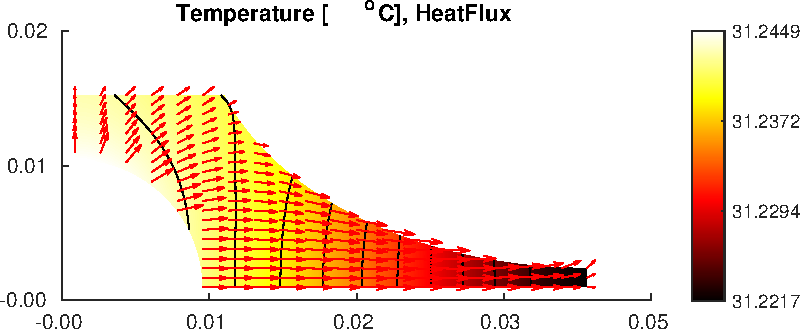
\includegraphics[width=0.8\textwidth]{flux_10.pdf}
%  \caption{Rozložení reploty pro průřez podobný optimálnímu.}
% \end{figure}
% 
% 
% Na vnitřní hranici topení v kontaktu s topným médiem je předepsán konstantní tepelný tok $Q=30\ W/m/cm$,
% daný teplnými ztrátami budovy rozpočítanými na délku topení. 
% Na vnější hranici v kontaktu se vzduchem je předepsána konstantní teplota $u=21$\textcelsius.
% 
% Otázky:
% \begin{itemize}
%  \item Jaký průřez je lepší?
%  \item Jak spočítat rozložení teploty na profilu, zejména na vnitřní hranici?
%  \item Je požadovaná teplot média dosažitelná?
%  \item Jak úlohu přesně formulovat matematicky?
%  \item Je úloha správně formulovaná, t.j. odpovídá fyzikální realitě?
% \end{itemize}
% 




% 
% 
% \subsection{Proudění v porézním prostředí}
% Uvažujme porézní prostředí, kde podíl pórů v referenčním objemu je $\nu$ $[-]$. Tuto bezrozměrnou veličinu nazýváme porozita. 
% Podíl tekutiny (vody) v referenčním objemu $\theta$ $[-]$ se nazývá saturace (opět bezrozměrná). Saturace se pohybuje od nějaké minimální (reziduální)
% saturace $\theta_r$ po saturovaný podíl tekutiny $\theta_s$ obvykle rovný porozitě $\nu$. Pro tekutinu se zachovává její hmota, resp. hustota v prostoru
% $\rho_V = \rho \theta$, 
% kde $\rho$ je hustota tekutiny. V nejjednodušším případě uvažujeme nestlačitelnou kapalinu, plně saturovné porézní prostředí
% a uvažujeme malé tlaky. V tom případě je $\rho$ i $\theta$ konstanta. Pak z obecné rovnice kontinuity dostaneme:
% \[
%     -\div \vc j = f,
% \]
% kde $\vc j$ $[kg/m^2/s]$ je hustota toku tekutiny  a $f$ $[kg/m^3/s]$ je hustota objemových zdrojů tekutiny. Podobně jako v případě tepla 
% je nejjednodušší vztah pro $\vc j$ dán gradientem tlaku $p$ $[Pa]=[kgm^2/s]$ pomocí tzv. Darcyho zákona:
% \[
%     \vc j = -\rho k\tn K \grad p.
% \]
% Zde $k=\kappa/\mu$ je hydraulická vodivost daná permeabilitou $\kappa$ $[m^2]$, která je vlastností porézního média, a viskozitou $\mu$ $[Pa.s]$, 
% která je vlastností tekutiny. Tenzor $\tn K$ je jednotkový v případě izotropního prostředí, ale v případě anisotrpního prostředí je to obecně symetrický 
% pozitivně definitní tenzor. Pokud má porézní materiál nějak orientované mikroskopické kapiláry, bude v jednom směru mít větší vodivost než ve směrech kolmých. 
% Obecně může mít materiál tři různé vodivosti ve třech různých směrech $k_x$, $k_y$, $k_z$ a nakonec tento materiál může být libovolně natočen v prostoru 
% pomocí matice rotace $Q$:
% \[
%     \tn K = \tn Q^T \tn D \tn Q,\quad 
%     \tn D = \begin{pmatrix}
%                 k_x     &0      &0\\
%                 0       &k_y    &0\\
%                 0       &0      &k_z                
%             \end{pmatrix}
% \]
% Vodivosti v hlavních směrech jsou vlastní čísla matice $\tn K$, musí být kladné. Matice rotace $\tn Q$ je tvořena (ortogonálními) vlastními vektory.
% Zde máme příklad anisotropie hydrulické vodivosti. Podobně existují materiály s anisotropní tepelnou vodivostí, nebo anisotrponí pevností etc.
% 
% Dále můžeme uvažovat stlačitelnou tekutinu, resp. stlačitelný materiál okolo pórů. Pro použití rovnice kontinuity pořebujeme spočítat derivaci 
% hustotu hmoty tekutiny v prostoru podle času:
% \[
%     \prtl_t \rho_V = \Big(\frac{\prtl \rho}{\prtl p} + \frac{\prtl \theta}{\prtl p}\Big)\prtl_t p = S\prtl_t p.
% \]
% Veličina $S$ $[kg/m^3/Pa]$ se nazývá storativita a zahrnuje jak stlačitelnost tekutiny $\prtl_p \rho$ tak stlačitelnost prostředí $\prtl_p \theta$.
% Pro nasycené, stlačitelné porézní prostředí tedy máme rovnici:
% \[
%     S \prtl_t p -\div\Big( \rho k\tn K \grad p\Big) = f
% \]
% 
% Pro nenasycené prostředí pak dostáváme záporné (sací) tlaky $p$ a pro ně saturaci $\theta_r \le \theta(p) \le \theta_s$, která je funkcí tlaku. 
% Navíc i vodivost $k$, klesá s klesajícím nasycením, je tedy $k(\theta)$ funkcí saturace. Dohromady dostaneme tzv. Richardsovu rovnici:
% \[
%     \prtl_t \theta(p) -\div\Big( \rho k(\theta(p)) \tn K \grad p\Big) = f
% \]
% kde funkce $\theta(p)$ a $k(\theta)$ jsou obecně nelineární a dostáváme tak nelineární parciální diferenciální rovnici.
% 
% 
% 
% \subsection{Transport chemických látek}
% \begin{equation}
%     \prtl_t (\rho_i c_i) + \div (\rho_i c_i \frac{\vc u}{\nu}) - \div( \tn D \grad c_i) = r_{ij}.
% \end{equation}
% 
% 
% \section{Vlnová rovnice (akustika)}
% 
% Odvodíme rovnici pro kmitání struny. Stav struny v čase $t$ a poloze $x$ je dán výchylkou struny $u(t,x)$. Pro zjendodušení si představujeme, 
% že struna může kmitat jen v jednom směru. Na element daný intervalem $(a,b)$ působí síly v koncových bodech:
% \[
%     \vc F(t,a) = -T(t,a) \vc t(t,a),\quad \vc F(t,b) = T(t,b) \vc t(t, b)
% \]
% kde $T$ je napětí ve struně a $\vc t$ je tečný vektor $ t(t, x) = ( 1, \prtl_x u(t,x) )$. 
% Jelikož v horizontálním směru se struna nepohybuje můsí být horizontální složka součtu sil rovna nule:
% \[
%     T(t,b) - T(t,a) = 0
% \]
% a jelikož jsme body $a$ a $b$ volili libovolně,  je napětí ve struně nazávislé na poloze: $T(t, x) = T(t)$.
% Proto pro vertikální složku síly platí 
% \[
%     F_y = F_y(t,a) + F_y(t,b) = T(t)\big(\prtl_x u(t,b) - \prtl_x u(t,a)\big)
% \]
% Nyní použijeme 2. Newtonův zákon:
% \[
%     \frac{\d}{\dt} \int_a^b \rho(x) \prtl_t u(t,x) \d x = F_y(t,x) = T(t)\big(\prtl_x u(t,b) - \prtl_x u(t,a)\big) = T(t) \int_a^b \prtl_{xx} u(t,x) \d x 
% \]
% A jelikož $a$ a $b$ jsou libovolné, dostáváme bodovou rovnici:
% \[
%     \rho(x) \prtl_{tt} u(t,x) = T(t) \prtl_{xx} u(t,x) 
% \]
% Pokud předpokládáme konstantní hustotu $\rho(x) = \rho_0$ a zanedbáme změnu napětí struny při malé výchylce $T(t)=T_0$ dostaneme vlnovou rovnici ve tvaru:
% \[
%     \prtl_{tt} u(t,x) = c^2 \prtl_{xx} u(t,x)
% \]
% kde 
% \[
%     c=\sqrt{\frac{T_0}{\rho_0}}
% \]
% je rychlost šíření vlny. 
% Mírně kompplikovanější je odvození vlnové rovnice pro změny (akustického) tlaku v prostoru:
% 
% \[
%     \prtl_{tt} p(t, \vc x) = c^2 \Lapl p(t, \vc x)
% \]
% kde pro rychlost zvuku $c$ platí:
% \[
%     c = \sqrt{\frac{B}{\rho_0}},\quad B = \rho_0 \frac{\prtl P}{\prtl \rho}
% \]
% přičemž $B$ je objemová stlačitelnost při adiabatické expanzi. Pro vzduch máme $B=1.45\times 10^5\ Pa$ a hustotu $\rho_0 = 1.2kg/m^3$ a dostáváme rychlost zvuku:
% \[
%     c=347 \sqrt{\frac{kg.m/s^2/m^2}{kg/m^3}} = 1251 km/h
% \]
% Tabulková hodnota je $340m/s$.
% 
% 
% 
% 
% 
% 
% 
% 
% \section{Mechanika}
% \dots
% \section{Elektromagnetismus}
% 
% \section{Klasifikace PDR}
% 






\subsection{Transportní procesy}
TODO: sloučit s předchozím

Rovnice vedení tepla odvozená v předchozí kapitole je jedním z příkladů transportních procesů, které popisují transport nějaké veličiny a
jsou odvozené ze zákona jejího zachování. Uvedeme pár dalších příkladů.

\subsubsection{Proudění v porézním prostředí}
Uvažujme porézní prostředí, kde podíl pórů v referenčním objemu je $\nu$ $[-]$. Tuto bezrozměrnou veličinu nazýváme porozita. 
Podíl tekutiny (vody) v referenčním objemu $\theta$ $[-]$ se nazývá saturace (opět bezrozměrná). Saturace se pohybuje od nějaké minimální (reziduální)
saturace $\theta_r$ po saturovaný podíl tekutiny $\theta_s$ obvykle rovný porozitě $\nu$. Pro tekutinu se zachovává její hmota, resp. hustota v prostoru
$\rho_V = \rho \theta$, 
kde $\rho$ je hustota tekutiny. V nejjednodušším případě uvažujeme nestlačitelnou kapalinu, plně saturovné porézní prostředí
a uvažujeme malé tlaky. V tom případě je $\rho$ i $\theta$ konstanta. Pak z obecné rovnice kontinuity dostaneme:
\[
    -\div \vc j = f,
\]
kde $\vc j$ $[kg/m^2/s]$ je hustota toku tekutiny  a $f$ $[kg/m^3/s]$ je hustota objemových zdrojů tekutiny. Podobně jako v případě tepla 
je nejjednodušší vztah pro $\vc j$ dán gradientem tlaku $p$ $[Pa]=[kgm^2/s]$ pomocí tzv. Darcyho zákona:
\[
    \vc j = -\rho k\tn K \grad p.
\]
Zde $k=\kappa/\mu$ je hydraulická vodivost daná permeabilitou $\kappa$ $[m^2]$, která je vlastností porézního média, a viskozitou $\mu$ $[Pa.s]$, 
která je vlastností tekutiny. Tenzor $\tn K$ je jednotkový v případě izotropního prostředí, ale v případě anisotrpního prostředí je to obecně symetrický 
pozitivně definitní tenzor. Pokud má porézní materiál nějak orientované mikroskopické kapiláry, bude v jednom směru mít větší vodivost než ve směrech kolmých. 
Obecně může mít materiál tři různé vodivosti ve třech různých směrech $k_x$, $k_y$, $k_z$ a nakonec tento materiál může být libovolně natočen v prostoru 
pomocí matice rotace $Q$:
\[
    \tn K = \tn Q^T \tn D \tn Q,\quad 
    \tn D = \begin{pmatrix}
                k_x     &0      &0\\
                0       &k_y    &0\\
                0       &0      &k_z                
            \end{pmatrix}
\]
Vodivosti v hlavních směrech jsou vlastní čísla matice $\tn K$, musí být kladné. Matice rotace $\tn Q$ je tvořena (ortogonálními) vlastními vektory.
Zde máme příklad anisotropie hydrulické vodivosti. Podobně existují materiály s anisotropní tepelnou vodivostí, nebo anisotrponí pevností etc.

Dále můžeme uvažovat stlačitelnou tekutinu, resp. stlačitelný materiál okolo pórů. Pro použití rovnice kontinuity pořebujeme spočítat derivaci 
hustotu hmoty tekutiny v prostoru podle času:
\[
    \prtl_t \rho_V = \Big(\frac{\prtl \rho}{\prtl p} + \frac{\prtl \theta}{\prtl p}\Big)\prtl_t p = S\prtl_t p.
\]
Veličina $S$ $[kg/m^3/Pa]$ se nazývá storativita a zahrnuje jak stlačitelnost tekutiny $\prtl_p \rho$ tak stlačitelnost prostředí $\prtl_p \theta$.
Pro nasycené, stlačitelné porézní prostředí tedy máme rovnici:
\[
    S \prtl_t p -\div\Big( \rho k\tn K \grad p\Big) = f
\]

Pro nenasycené prostředí pak dostáváme záporné (sací) tlaky $p$ a pro ně saturaci $\theta_r \le \theta(p) \le \theta_s$, která je funkcí tlaku. 
Navíc i vodivost $k$, klesá s klesajícím nasycením, je tedy $k(\theta)$ funkcí saturace. Dohromady dostaneme tzv. Richardsovu rovnici:
\[
    \prtl_t \theta(p) -\div\Big( \rho k(\theta(p)) \tn K \grad p\Big) = f
\]
kde funkce $\theta(p)$ a $k(\theta)$ jsou obecně nelineární a dostáváme tak nelineární parciální diferenciální rovnici.



\subsubsection{Transport chemických látek}
\begin{equation}
    \prtl_t (\rho_i c_i) + \div (\rho_i c_i \frac{\vc u}{\nu}) - \div( \tn D \grad c_i) = r_{ij}.
\end{equation}










%\section{Mechanika}
%\dots
%\section{Elektromagnetismus}

\subsection{Klasifikace PDR}

\subsubsection{Eliptické rovnice}
Základním příkladem je Laplaceova rovnice:
\[
    \Lapl u(\vc x) = 0
\]
respektive Poisonova rovnice
\[
    \Lapl u(\vc x) = f(\vc x).
\]
Dalšími příklady je stacionární rovnice vedení tepla:
\[
    \div( k \grad T(\vc x) ) = f(\vc x),
\]
resp. stacionární rovnice Darcyho proudění:
\[
    \div( \tn K \grad p(\vc x)) = f(\vc x).
\]
Obecná rovnici druhého řádu:
\[
  \div\Big( \tn A \grad u(\vc x)\Big) + \vc b \grad u(\vc x) + c u(\vc x)= f(\vc x)
\]
je eliptická, pokud $\tn A$ je symetrická pozitivně definitní matice.

Pro eliptické rovnice platí (za jistých omezeních pro $\vc b$ a $c$) tzv. princip maxima. Pokud $u$ je řešením eplitické rovnice na oblasti $\Omega$
pak 
\[
    \max_{\vc x \in \Omega} u(\vc x) \le \max_{\vc x \in \prtl \Omega}  u(\vc x).
\]
Podobně pro minimum:
\[
    \min_{\vc x \in \Omega} u(\vc x) \ge \min_{\vc x \in \prtl \Omega}  u(\vc x).
\]


\subsubsection{Hyperbolické rovnice}

Příklad je vlnová rovnice:
\[
    \prtl_{tt} p(t, \vc x) = c^2 \Lapl p(t, \vc x)
\]

Transportní rovnice (rovnice kontinuity), např. pro rozpuštěnou látku:
\[
    \prtl_t (\rho c) + \div( (\rho c) \vc u)=0
\]

Eulerovy rovnice:
\[
    \prtl_t \rho + \div( \rho \vc u)=0
\]
\[
    \prtl_t (\rho \vc u_i) +\div(\rho \vc u_i \vc u) = - \grad P,
\]
Kvalitativní vlastnosti řešení:
\begin{itemize}
 \item Konečná rychlost šíření (vln).
 \item Nezhlazuje.  
 \item Nesplňuje princip maxima, řešení se může akumulovat v bodě (náraz vlny na pobřeží).
\end{itemize}


